\chapter{Literature Review}
\label{ch:background}

In this chapter, we present previous works that investigated the effect of 
computational environments on scientific results: we provide results 
that show the magnitude of the effect of computing environment changes such 
as hardware and software implementations. Next, we review 
techniques and tools to enhance the reproducibility of the experiments 
including code and data sharing methods using version control 
systems, and virtualization techniques to encapsulate computational 
variability of the analysis. 
% We presents the role that numerical stability plays in these problems 
% several case studies in neuroimaging to demonstrate the necessity of
% exploring numerical stability in this space.
Finally, provenance management tools are described 
to collect and represent the analysis dependencies. 


\section{Computational Reproducibility}

There have been many works investigating the reproducibility of
computational pipelines in the past few years. In general, analysis 
results are not reproducible across small perturbations of the 
execution environments, including hardware configuration or operating 
system. 

Changes in the computational environment may introduce small numerical 
errors, subsequently propagated and amplified by pipelines. In this 
case, the analysis pipelines are said to be numerically unstable. 
Numerical instability is a characteristic of the pipelines which 
amplify small numerical errors and then hamper the reproducibility 
of the analyses depending on the length of the pipeline and magnitude 
of the errors. In many cases, numerical instability is an important 
issue for reproducibility. 

The following sections will discuss the effect of influential elements on 
reproducibility, in particular workstation type, parallelization techniques, 
operating system changes, analysis software variety, and perturbations 
applied in input data. 

\subsection{Effect of Hardware Resources}

The hardware configuration of computers has been detected as an 
influential source of irreproducibility~\cite{hill2017numerical}. Such 
differences are particularly noticeable across computing processors 
such as CPUs (Central Processing Units), GPUs (Graphics Processing 
Units) and APUs (Accelerated Processing Units), mainly due to conflicts 
of floating point units (FPU) with the IEEE-754 standard when 
arithmetic precision of the floating-point values are not specified 
uniformly.

Even using the same arithmetic precision, it is difficult to achieve 
bitwise identical results across different hardware resources. 
Recent studies show that hardware developments to improve 
computational performance sacrifice numerical 
reproducibility~\cite{duben2014use, demmel2013numerical}. For instance, 
code optimization techniques embedded inside the CPUs, known as 
out-of-order execution (dynamic scheduling) paradigm, impede the 
reproducibility. In this paradigm, the processors might execute 
instructions out of the original order they appear based on the 
availability of input data and execution units to use resources 
efficiently~\cite{wiki2018out-of-order}. Therefore, it might compute 
floating-point operations in different order, which often leads to 
different results. In this case, 
these papers~\cite{duben2014use, demmel2013numerical} 
showed that some operations in 
particular sum and division are not associative because of different 
rounding of the intermediate floating-point results.

Furthermore, the study in~\cite{jezequel2015estimation} implements 
acoustic wave equation to see the effect of processor architecture on 
results. The authors illustrate irreproducible results across 
different processors including AMD CPU, NVIDIA GPU, and AMD APU, even 
using the same IEEE-754 standard. The results numerically vary from one 
architecture to another, the maximal relative difference between 
results is of $10^{-1}$ to 1 and its mean value is $10^{-5}$. Such 
differences often occur due to rounding errors generated by different 
orders in the sequence of arithmetic operations. Indeed, this is 
already a challenge on today's platforms. 

In neuroimaging, it is important to evaluate the consistency of  
results when they are executed on a heterogeneous computing system. For 
this purpose, a number of tests were conducted 
in~\cite{Gronenschild2012} to gain insight into the variability of  
results from neuroimaging packages based on different data processing 
conditions like different workstation types. In this paper, two 
different types of workstations are compared: an HP (Hewlett Packard) one 
using Centos 5.3 and 8 CPU cores, and a Mac one using OSX 10.5.8 and 2 
CPU cores. This study shows significant absolute differences among 
the volumes of anatomical structures obtained on the two different 
workstations. 


\subsection{Effect of Parallelization}

Developers leverage parallelization techniques to accelerate the 
execution performance at different levels, from multi-threaded programming to 
high-performance computing (HPC). Within such computations, contrary to 
sequential implementations, the execution order of the processes may 
change in different runs. Consequently, several runs of the 
parallelized code may produce different 
results, even on the same computer. 

To show the existence of such issues, the impact of the number of 
processors on numerical reproducibility is studied 
in~\cite{diethelm2012limits}. This study simulated the process of 
deformation of metal sheets in the packaging industry to measure local 
change of the sheet thickness using different number of processors. 
Results obtained different sheet thicknesses, which shows the 
amplification of rounding errors in summations after running the same 
simulation on the same computers with different number of processors. 
This proved that summation operation is not associative because of 
different rounding of the intermediate floating-point results, even 
using the standard IEEE double-precision arithmetics. Therefore, final 
result of the summation depends on the order in which values are 
processed which could be changed by the number of processors. 

Another statistical simulation showed reproducibility failures in 
multi-core processing performed on GP-GPUs and multi-core 
CPUs~\cite{taufer2010improving}. Multi-core architectures enable 
multi-threaded environment for running numerical intensive applications 
at high speeds. This study showed that the stability of molecular 
dynamics simulation results is not guaranteed in multi-core processors 
due to using different order of floating-point operations (e.g. 
division and square root operations) in ways that these operations lead 
to different rounding and truncation. 

In addition, parallel programming may lead to race conditions that 
further impede reproducibility. A race condition is a situation in 
concurrent programming where two concurrent threads or processes have 
access to the same resources and attempt to change it at the same time. 
When one thread is performing read on a particular data element, 
another thread is allowed to modify or delete this element. So, the 
resulting final state depends on the order of process operations, which 
is not specified by the application. In addition to race condition, 
some other problems have been listed as the main sources of numerical 
differences in many paralelized experiments such as out-of-order 
execution, and message buffering non-blocking communication 
operations~\cite{revol2013numerical}. 

Message buffering is a type of communication using send/receive 
functions in parallel programming, which can be blocking and 
non-blocking. In contrast to blocking, non-blocking communication do 
not block process if the communication is not finished yet. 
Non-blocking means that computing and transferring data can happen in 
the same time for a single process. This allows communication to 
overlap, which generally can leads to different computing order and 
irreproducible results for different runs. 

Furthermore, some experiments are reported in~\cite{Gronenschild2012} 
to determine the effect of parallelization on neuroimaging pipelines, 
most precisely in different versions of FreeSurfer. Regarding these 
experiments, results demonstrate that concurrent running would not make 
statistical significant differences based on the comparison of voxel 
volume of specific brain structures for the same conditions. This is an 
example where Peng's reproducibility is achieved while numerical 
reproducibility is not.

\subsection{Effect of Operating System}

In this section, we summarize the results of the work in~\cite{Glatard2015}, 
which quantified the reproducibility of computational analyses 
across operating systems. In particular, the authors determined 
the reproducibility of three neuroimaging workflow packages, FSL, 
FreeSurfer, and CIVET between CentOS 5.10 and Fedora 20. 

Using FSL package, cortical and subcortical tissue classifications 
resulted in minor differences between the classified tissues on CentOS 
and Fedora operating systems. These differences mainly correspond to 
the mathematical functions implemented in different operating system 
libraries. 

The results of \emph{RS-fMRI} analysis revealed significant inter-OS 
differences in the second experiment. This analysis showed that each 
pre-processing step can introduce small numerical variations, but their 
accumulation creates important differences. These numerical differences 
are caused by changing implementation of mathematical functions like 
\emph{sinf()} between operating systems.  

Using FreeSurfer and CIVET packages, cortical thickness extraction 
introduced important differences in some specific brain regions across 
the operating systems. Figure~\ref{inter_os} shows localized regions of 
these differences for CIVET, which are quantified by the metrics 
including mean absolute difference, standard deviation of absolute 
difference, t-statistic and random field theory (RFT). 

Additionally, inter-build differences are measured in this study. A 
static build of a pipeline refers to its compiled version where 
libraries are statically linked. In this test, the authors used the 
static builds of FreeSurfer CentOS 4 and CentOS 6 to measure their 
reproducibility. Results show that building static program improves 
reproducibility across OSes, but small differences still remained. The 
main cause of such differences is dynamic libraries that are loaded by 
the static executable at run-time. 

\begin{figure}[H]
\centering
	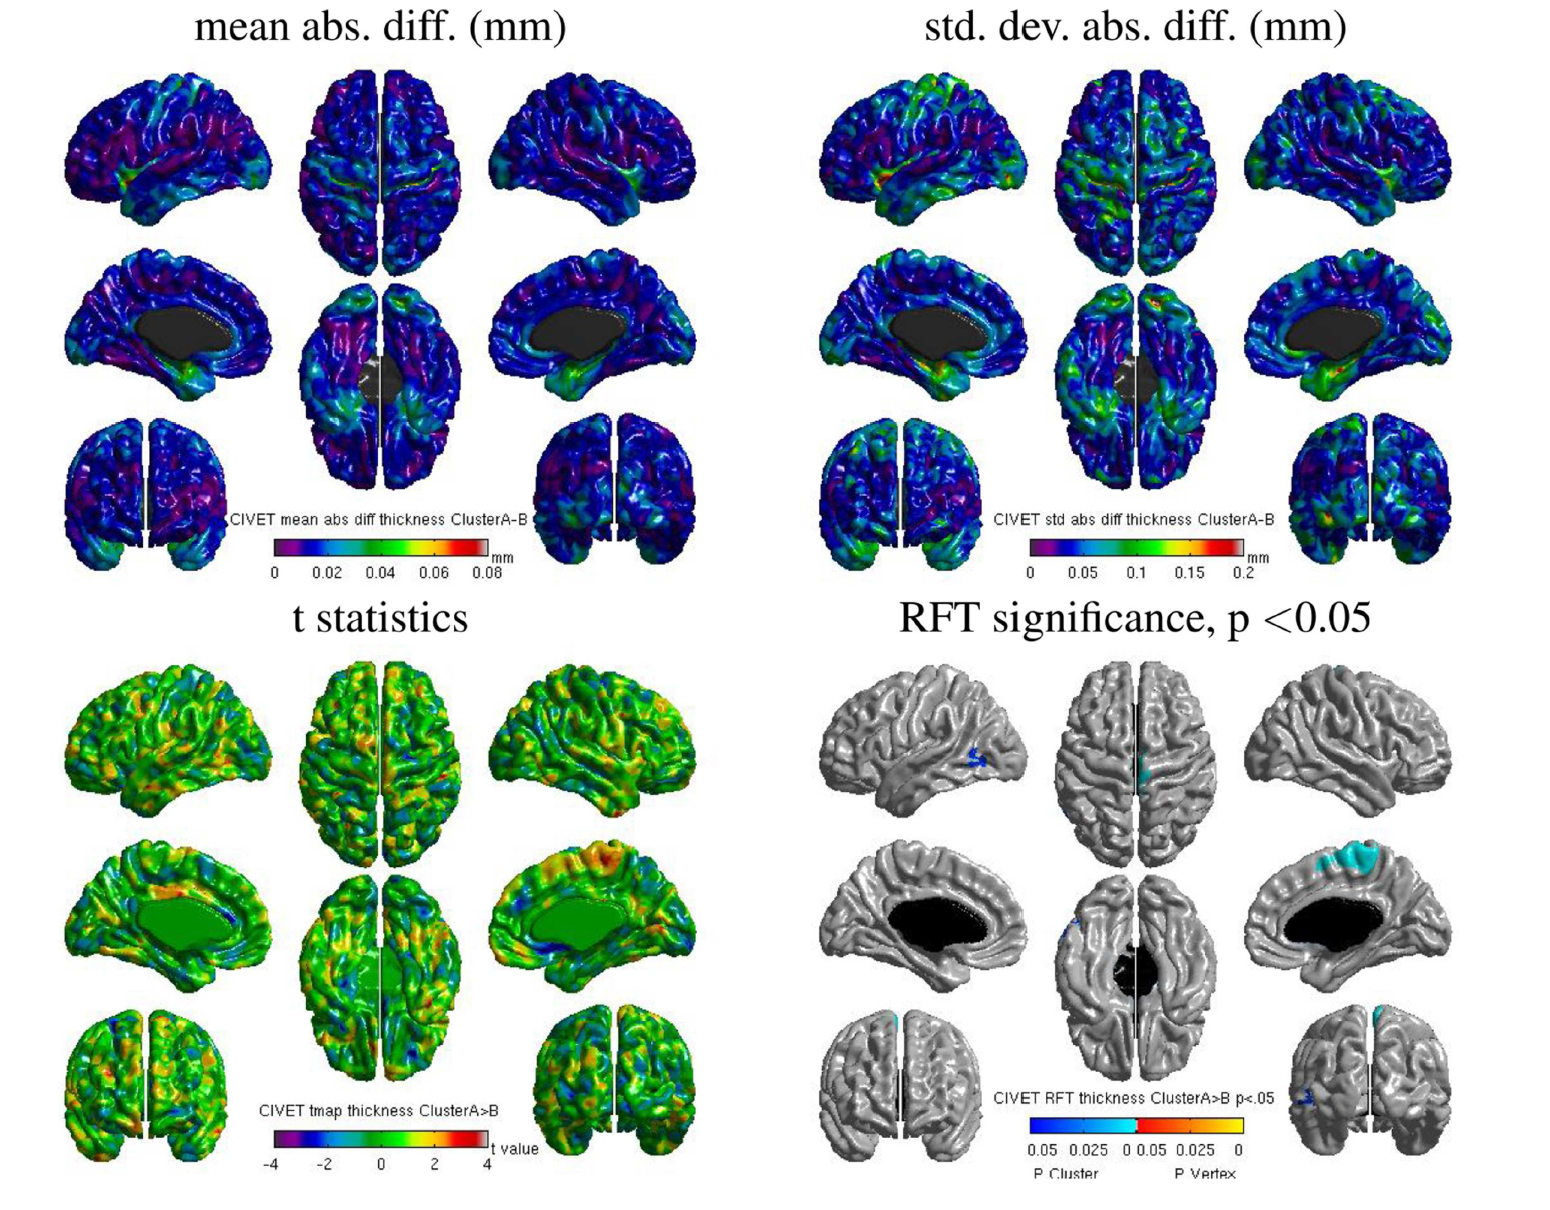
\includegraphics[scale=0.9]{chapters/background/images/inter-os-diff} 
	\caption{Surface maps of four metrics, standard-deviation and mean 
	absolute differences, t-statistic and RFT significance values, 
	indicate the inter-OS differences for the cortical thickness 
	extracted with CIVET over 146 subjects~\cite{Glatard2015}. } 
	\label{inter_os}
\end{figure}
 

In~\cite{Glatard2015}, it has been detected that most of the 
neuroimaging pipelines are sensitive to the operating 
systems. The effect-size of the variations is changed based on the 
complexity of the analysis pipeline. For instance, shorter analyses 
like brain extraction have much less significant disagreement compared 
to the longer ones like subcortical tissue classification and RSfMRI 
analysis.

Furthermore, the authors expect similar reproducibility issues for the 
other Linux distributions including Debian and Ubuntu as long as they 
are based on glibc, the GNU C library, which includes mathematical 
libraries. In addition, other studies~\cite{Gronenschild2012, 
Krefting2011} have reported similar issues for non-Linux operating 
systems. 


\subsection{Effect of Analysis Software}

Reproducibility of computations also depends on the executed analysis 
software, even using the same operating system and hardware resources. 
Different version of analysis software used in a computation may 
produce different results. Also, re-implementation of the same 
experiment through different software packages can introduce 
discrepancies in results. In this section, we summarize the impact of 
software variability including different software versions and a wider 
range of software packages on reproducibility of results. 

\subsubsection{Effect of software versions} 

In addition to comparing hardware and operating system variability 
in~\cite{Gronenschild2012}, the impact of using different pipeline 
versions is investigated.
Significant volume differences are quantified across the FreeSurfer 
versions for both anatomical brain structures and cortical thickness 
measures. Thus, it is important for users to be able to reproduce 
analyses in any future update of these analytic software. 

Moreover, the same study~\cite{Gronenschild2012} showed that the effect 
size of different operating systems or software versions are close to 
the ones measured in neuropsychiatric diseases. For example, the impact 
of Alzheimer disease and semantic dementia on Grey Matter volume 
changes are reported in~\cite{lehmann2010atrophy}. These results show 
similar changes between volumes of specific structures in compared to 
the discrepancies caused by computation environment variability 
in~\cite{Gronenschild2012}. In addition, differences in cortical 
thickness caused by various operating systems, software versions and 
workstation types were roughly of the same order of magnitude than the 
findings reported in~\cite{kuperberg2003regionally} from patients who 
suffered from schizophrenia. There are many other proofs in different 
domains that show the influence of software updates on  
results~\cite{shim2015effect, wadi2016impact}.

\subsubsection{Effect of software packages} 
\label{swf_effect}

In all aforementioned analyses, the choice of the software package 
remained fixed for carrying out the analyses in each study. To figure 
out the impact of analysis software variations on task fMRI results, 
several tests were conducted in~\cite{bowring2019exploring}. They 
investigated differences produced across three of the most popular 
neuroimaging software packages, AFNI, FSL, and SPM. They replicated 
specific analyses, a number of image processing steps, as closely 
matched to the original study as possible. 

The statistical comparisons show a substantial disagreement between 
software package results such as producing different location of 
activation regions. 
Figure~\ref{inter_sfw} shows the substantial variation 
between each main activation area found in the original study and the 
reanalyses. Results indicate that the precise location of the significant 
activated regions is highly dependent on the choice of software package 
and inference method.

\begin{figure}[H]
\centering
	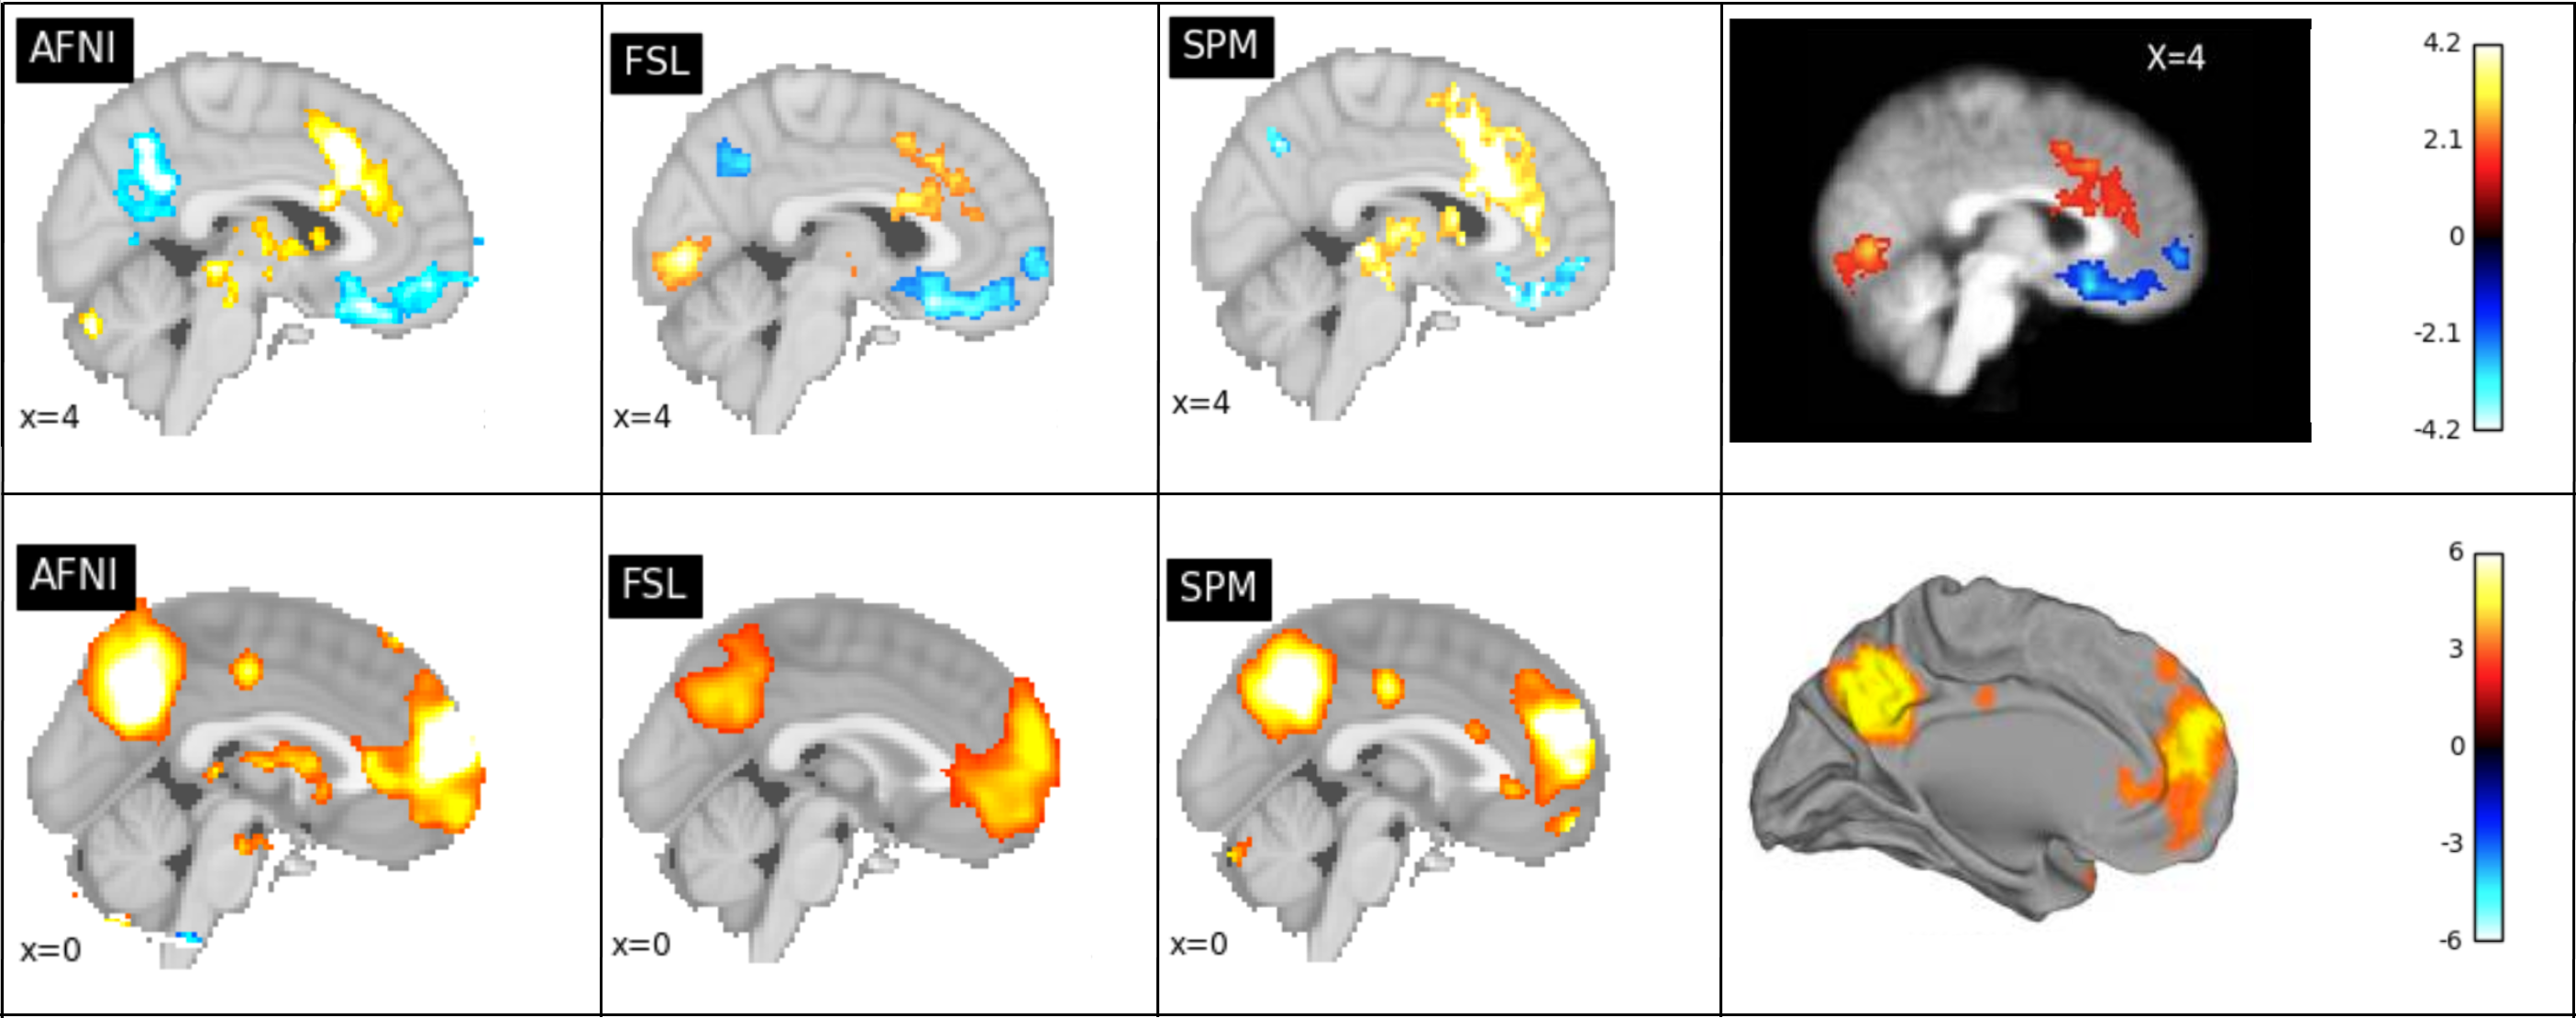
\includegraphics[scale=0.5]{chapters/background/images/inter_sfw} 
	\caption{Comparison of the thresholded statistic maps of two 
	different analyses within AFNI, FSL and SPM. Each row shows the 
	results of each reanalyses, and the last column shows the main 
	figure from the original publication. Total 16 subjects and 21 
	subjects are participated in the first study (first row) and second 
	study (second row) respectively~\cite{bowring2019exploring}.
	\label{inter_sfw}}
\end{figure}

In addition, from the analyses conducted 
in~\cite{bowring2019exploring}, it is found that the size of datasets 
can contribute to the variation of results. For instance, results 
obtained from analyses that use smaller sample size are less likely to 
be reproducible than analyses in which more subjects are participated. 
Therefore, variation in the outcome of an fMRI analysis depends not 
only on the choice of software package used, but also on the dataset 
being analyzed. 


\subsection{Effect of Small Data Perturbations}

It has been shown in the previous sections that neuroimaging pipelines 
are sensitive to changes in the computing environment. More precisely, 
a few studies were conducted to show the instability of some specific 
steps of MRI analysis through the simulation of minor perturbations in 
input data. For instance, reproducibility of the cortical surface 
reconstruction analysis in the presence of small perturbations is 
measured in~\cite{Lindsay2017hbm}. They investigated results of two 
pipelines, CIVET and FreeSurfer, after applying 1\% intensity 
modification on one voxel located in a non-cortical region. Contrary to 
expectations, widespread surface changes were observed across the 
cortex. 

Similarly, another study~\cite{Glatard2018hbm} observed substantial 
variability of motion correction algorithms in fMRI analyses by 
applying one-voxel perturbation. Results demonstrate significant 
differences specifically for Niak and FSL packages in this study. These 
variations may result in wrong activation maps and increase the 
prevalence of false activations on the subsequent steps of fMRI 
processing. 

Recently, processing of high-resolution images are made possible 
through a new version of pipelines. Therefore, the study 
in~\cite{Lindsay2018hbm} quantifies the variability of analysis results 
across different image resolutions. The authors investigated the 
partial volume effects of various image resolutions on the automated 
cortical surface extraction through CIVET and FreeSurfer pipelines. 
This study shows a significant variability on results for the same 
analysis using images with different resolutions. For both pipelines, 
mean absolute error, signed error, and standard deviation are mostly 
reduced as a function of increasing resolution. Also, comparison of 
projected distance error maps between histological ground truth 
surfaces and MRI-derived surfaces confirms that the accuracy of 
analysis is increased in higher resolutions. Further research is needed 
to minimize partial volume effects along with magnifying the resolution 
to get a more accurate results. 

% \subsection{Conclusion}

% We reviewed reproducibility of the computational analyses across data 
% perturbations and different computing environments such as operating 
% system, workstation type, software version, etc. We found that these 
% elements have significant effects so that would change the results of 
% analyses. So, reproducibility of analysis is highly dependent on 
% computational environments. Also, it should be noted that the influence 
% of all these elements are of the same importance and each of them 
% cannot be more important than other one. 

% We investigate reproducibility of analyses across small perturbations. 
% Therefore, the choice of analysis software remained fixed to assess the 
% reproducibility issues across a number of computational parameters in 
% my research. In this way, we can determine reproducibility issues 
% caused by the pipeline instability. Accordingly, we will introduce 
% several solutions to address such reproducibility issues in the next 
% chapter. 

\section{Techniques to Improve Reproducibility}
\label{techniques}

Reproducibility is mainly ensured through three properties, including 
source sharing for both code and data, 
research portability, and pipeline 
stability. Source sharing and research portability can be related to 
the FAIR principles~\cite{wilkinson2016fair} according to which 
scientific sources have to be findable, accessible, interoperable, and 
re-usable. 

First step in reproducibility is to find and access research products, 
which is related to Findable and Accessible principles in FAIR. 
Code and data must be publicly available in a 
machine-readable structure. It enables the verification of scientific 
results by independent investigators. Therefore, reproducibility 
increases the reliability and transparency of experiments. 

Through reproducibility, analysis pipelines need to be able to 
integrate with other execution environments. This is termed research 
portability, and can be achieved using virtual machines and 
containerization technologies. Portability enables researchers to 
re-run analyses in a variety of execution conditions. This can be 
matched with the Interoperability and Re-usability of FAIR principles. 

In addition, analysis pipelines must be numerically stable across a 
variation of the computing environments to be reproducible. Although 
many solutions currently exist to address analysis sharing and 
portability, the effect of numerical instability remains largely 
unexplained. In this chapter, we will discuss a number of techniques 
and tools used to enhance sharing, portability, and stability of the 
analysis.


\subsection{Code and Data Sharing}

To successfully reproduce a computational experiment, analysis sources 
must be accessible in a machine-readable 
structure~\cite{stodden2016enhancing,hasham2018cloud}. The importance 
of a proper structure is clear, specifically when we aim to share 
codes with others or contribute to a wider group.

One foundation of code sharing is modern software engineering, which 
includes practices like version control systems (VCS). Version control 
ensures that history of the code is available and archived. 
Git~\cite{git}, as one of the most popular VCS frameworks, provides a 
distributed platform to manage project files. Git facilitates the 
collaboration of developers on the same project using GitHub. GitHub is 
a web-based service for Git, which hosts repositories. 

Sometimes developers tend to share programs instead of source code 
because of commercial reasons, simplifying its usage, reproducibility, 
etc. For this purpose, several sharing tools exist that maintain a set 
of packages. As an example of more generic sharing tools, PyPI (Python 
Package Index) is a software repository for the Python programming 
language. PyPI helps to share python packages, and allows users to 
search for packages by keywords. Futhermore, there are more specific 
sharing tools for neuroimaging programs including 
Boutiques~\cite{glatard2017boutiques}, a system to publish and 
integrate command-line applications automatically using a JSON 
descriptor across computational platforms, or 
NITRC-CE~\cite{kennedy2016nitrc} which provides a number of 
pre-installed neuroimaging tools such as AFNI, FSL, and FreeSurfer into 
a standardized computational environment. 

Furthemore, data sharing is important as it facilitates reproducibility 
of analyses, and it enables the assessment of future works in 
comparison with previous analyses. However, there are some challenges 
associated with data sharing including concerns about the privacy of 
personal information, lack of incentive by other researchers, and 
technical issues associated with sharing of large datasets. 

Git is a very efficient tool for managing textual information such as 
code, text, and configuration, but it is inefficient for storing large 
data. Therefore, extensions of Git named git-annex~\cite{git-annex} 
and Git-LFS (Large File Storage)~\cite{git-lfs} were developed to 
address the problem of sharing and versioning large data collections. 
git-annex uses Git to store and index files without committing large 
files into the Git repository. Similarly, Git-LFS reduces the impact of 
file size in repository by replacing large files with lightweight 
pointer files in the repository, which refer to the actual file 
location. 

Both Git and git-annex are great for collaboration on a single 
repository, but sharing code and data between multiple projects can be an 
issue across these tools. Also, they lack advance meta-data search 
capabilities. For instance, they cannot crawl throughout domain-specific repositories.
 For this purpose, Datalad~\cite{datalad} is an 
efficient tool particularly for data sharing and versioning across 
multiple datasets. This tool is built on top of the git-annex and provides 
unified access to data regardless of its origin. There is a guarantee 
that the content for the same version would be the same across all 
clones of dataset, regardless where content was obtained from. 
DataLad supports multiple redundant data providers for each file in a 
dataset, and will transparently attempt to obtain data from an 
alternative location if a particular data provider is not available. 
Furthermore, a provenance record is provided by Datalad with all 
necessary information about input data to reproduce the analysis 
results. 

In addition, higher level platforms were designed to help 
scientists share neuroimaging data and make them public on web such as 
openNeuro~\cite{gorgolewski2017openneuro}, LORIS~\cite{das2012loris}, 
and XNAT~\cite{marcus2007extensible}. 
These tools usually have a web-based user-friendly interface, and can 
integrate with processing platforms. Also, Most of these tools use the 
Brain Imaging Data Structure (BIDS)~\cite{gorgolewski2016brain} to 
describe and organize neuroimaging data. BIDS specification provides a 
standard for organizing and representing MRI data that reduces the 
effort of data sharing. 

Moreover, there exists a number of projects that promote open 
data-sharing initiatives in the field of neuroimaging including the 
International Neuroimaging Data-Sharing Initiative 
(INDI)~\cite{mennes2013making, milham2012open}, the Alzheimer’s Disease 
Neuroimaging Initiative (ADNI)~\cite{jack2008alzheimer}, and Human 
Connectome Project (HCP)~\cite{van2012human}. Using data published by 
these projects, researchers who once struggled to access to the 
restricted datasets can now explore thousands of published subjects. 
Public access to this amount of brain imaging data has become 
invaluable for specialists to test a variety of scientific hypothesis 
and evaluate novel image processing algorithms. 


\subsection{Portability}

Given that source code and data used in the original experiment are 
available, re-executing a computational analysis is still not 
straightforward. To reproduce computational analyses, information about the
computing environment is needed, in particular the operating system 
configuration, the hardware system architecture, and specific versions of 
tools. Therefore, virtual machines and containerization techniques are 
suggested to ensure that specific computing parameters are completely 
preserved. 

Virtual machines (VMs) can be used to encapsulate the entire context of 
computations, which provides an exact replica of the computational 
environment where analyses took place. The most popular implementations 
of VMs include VMware~\cite{wiki:vmware}, 
VirtualBox~\cite{watson2008virtualbox}, and KVM~\cite{kivity2007kvm}. 
VMs may produce large images because they hold a copy of all the 
operating system files including kernel, system libraries, and system 
configuration files. In addition, VMs bring an extra 
performance overhead such as I/O, CPU, and memory.

In contrast, containerization tools like 
Docker~\cite{boettiger2015introduction} and 
Singularity~\cite{kurtzer2017singularity} reduce dramatically the 
performance overhead and image size of VMs by sharing the kernel of the 
host system across the containers. These tools have emerged to build 
lightweight and portable images. Container images can be version 
controlled in the same way as the analysis code so that the exact same 
computing environment can be used to re-execute an analysis. However, 
similar to VMs, users are faced with the burden of ensuring that all 
necessary dependencies are collected inside the containers. For this 
purpose, some workflow management systems are developed to record the 
computational dependencies: we will describe them in the next section. 

As an example of container-based tool, Nextflow~\cite{di2017nextflow} 
is implemented to ensure workflow reproducibility. Nextflow uses Docker 
to containerize pipeline dependencies including data, code, and the 
computing environment. Nextflow can be integrated with public 
repositories in GitHub and cloud computing infrastructures to provide a 
rapid computation and effective scaling. 

It should be noted that containers are excellent technologies to solve 
portability issues. However, they are not perfect solutions to address 
the reproducibility of analysis across computing environments because 
they mostly mask differences instead of fixing them, as explained hereafter.

\subsection{Numerical Instability}

Containers and VMs are good to mask the effect of hardware, 
paralellization, and operating system. However, it is very likely that 
this effect is due to numerical instabilities in the data analysis 
pipelines. We believe that these effects are the combined results of 1) 
the creation of numerical errors between conditions and 2) the 
amplification of these numerical errors throughout the pipelines. 

\subsubsection{Creation of Numerical Errors}

Main causes of numerically irreproducibility are the limitations of 
floating point operations, in particular, using a finite precision in 
their arithmetic operations like summation~\cite{hill2017numerical, 
taufer2010improving}. In this section, several solutions are proposed 
to improve numerical reproducibility related to the floating-point 
operation, but they would not fix numerical instability. 

Floating-point numbers are composed of a mantissa (significand) as the 
significant digits of the number, a base and an exponent that specifies 
the right finite precision, and a sign for both negative and positive 
values. Floating-point data type represents an approximation of a real 
number on computers, depending on the size of the 
mantissa~\cite{hill2017numerical}. Each computing system provides 
standardized math libraries necessary for the floating-point 
computations with a finite precision. However, finite precision 
computations create numerical errors mostly due to truncation error and 
round-off error. 

Truncation error is the error caused by truncating a mathematical 
procedure. Some computations include infinite number of terms for exact 
solutions like Taylor series and exponential functions. 
In numerical 
solution, we can only use a finite number of terms. Therefore, these 
functions will be truncated after a finite number of calculations to 
evaluate an approximation. This difference between a truncated value 
and actual value is called truncation error~\cite{kiusalaas2013numerical}. 

Round-off error, also called rounding error, is the error caused by 
approximate representation of numbers. Computers can represent 
floating-point numbers with a fixed number of digits (fixed precision). 
Therefore, they have to round numerical results to the closest number 
that they can represent, this is leading to rounding 
error~\cite{fadnavis1998some}. Although rounding error is in the order 
of $e>10^{-7}$ for single precision and $e>10^{-16}$ 
for double 
precision, their accumulation can be significant. 

Rounding errors can lead to different results depending on the order in 
which operations are performed. In particular, in the presence of 
rounding errors the addition is not associative. For instance, assuming 
a computer with 4 decimal digits of precision, the following summation 
in different orders leads to different results.
\[
(4.127 \oplus 100.2) \oplus -104.2 = 104.3 \oplus -104.2 = 0.100
\]
\[
4.127 \oplus (100.2 \oplus -104.2) = 4.127 \oplus -4.000 = 0.127
\]

In the first summation, rounding error would be introduced in the truncation of 104.327 to 104.3.
This shows rounding errors leading to different results, depending on the precision of floating-point numbers used by the system.
% In addition, rounding errors would lead to different results depending 
% on the precision of floating-point numbers used by the system.

To address these numerical errors, a number of 
solutions are proposed in~\cite{muller2018reproducible} 
such as using higher precision, deterministic order of operations, 
arbitrary-precision operations, and fixed-point arithmetic.

\paragraph{Higher precision.} Using high-precision numbers can yield 
reproducible results with high probability. For instance, calculations 
using double precision produce more accurate results than single 
precision. 
However, it is not a sufficient solution because  
tiny rounding errors still exist for the higher precision, which can 
produce significant bits flip (e.g. from 0.999999... to 1). 

\paragraph{Deterministic order of operations.} It is possible to make 
computations deterministic in terms of the order in which floating 
point operations are performed. This can result in reproducible results 
across runs, but this solution may add memory overhead, and affect 
the performance of executions. 

\paragraph{Fixed-point arithmetic.} Unlike the floating point numbers, 
fixed-point numbers reserve a fixed number of digits after the decimal 
point, regardless of how large or small the number is.
It is common to use fixed-point arithmetic to represent large 
fractional numbers. Although it helps to avoid of rounding errors, it 
limits range of values. Fixed-point operations are often slower than 
floating-point operations which are implemented in hardware like CPUs 
and GPUs.

\paragraph{Arbitrary-precision operations.} We can use high-precision 
or even arbitrary-precision operations to push the limits of 
fixed-point arithmetic. This means that the precision of numbers is 
limited only by the available memory of the host system. 
This not only requires many hardware instructions for each arithmetic 
operation, but also variable-width storage is much more difficult to 
handle than the fixed-width. 


\subsubsection{Amplification of Numerical Errors}

There is evidence showing that analyses are not stable to small numerical 
errors because of propagation and amplification of these errors. 
For instance, propagation of rounding errors from initial value in 
numerical computations were studied by performing different experiments 
in~\cite{fadnavis1998some}. In this paper several computational 
experiments are presented to demonstrate the rapid growth of rounding 
errors in iterative computations like iterative addition. The 
accumulation of rounding error from summation operation indicates that 
analyses may produce different results. Due to similar reasons, the 
propagation of rounding error when simulating the metal sheet thickness 
changes in~\cite{diethelm2012limits} turned to different results.

Another study~\cite{Glatard2018hbm} evaluates the stability of different 
neuroimaging pipelines in presence of one voxel perturbations. This 
study showed that iterative initialization schemes in motion correction 
algorithms lead to the propagation and amplification of numerical 
errors along the time series. 

To address the numerical instability of pipelines, we can use bootstrap 
technique. In~\cite{Glatard2018hbm}, the authors explained that bootstrapping 
is an efficient technique to improve the robustness of motion 
estimation. The bootstrap version of the pipelines computed the median 
transformation results from the 30 samples from the medians of the 
parameters of the 30 transformations. It is, however, a 
compute-intensive technique that should be used only when no other 
solution to the instability is available. 

In addition to bootstrapping, it is shown that bagging technique can 
reduces the effect of perturbations~\cite{breiman1996bagging, 
breiman1996heuristics}. Bagging, also called bootstrap aggregating, is 
a simple and powerful ensemble method. It helps reduce both bias and 
variance in the results. So, we can possibly stabilize pipelines and improve 
their accuracy using aggregates of results obtained with data 
perturbations. 


\section{Provenance Capture}

We discussed about portability of analyses as a necessary feature for 
reproducibility, which enables researchers to re-run analyses in a 
variety of execution conditions. Portability requires comprehensive 
information about the computational analysis in a machine-executable 
form. This information can be achieved by provenance capturing 
tools. 

Provenance is defined as the collected information about objects and 
processes involved in workflow result. This information can be 
used to verify reliability and reproducibility of 
executions~\cite{missier2013w3c}. Provenance information can contain the 
metadata that displays what data processing is 
undergone~\cite{nichols2017best}. For example, which parameters are 
used for the analysis, what form of image is used, how the image was 
registered/aligned to a standard space, how noise was eliminated, how 
an specific feature has recognized. Capturing such information is 
out of the scope of my research. Instead, we are looking for 
detail of the computing environments provided by the provenance 
capturing tools. In this chapter, we will discuss different aspects 
of provenance capturing such as system-level provenance capturing and 
workflow specifications. Finally, we give examples of some specific 
workflow engines that provide these features. 

\subsection{System-Level Provenance Management Tools}

Automated provenance capturing of computational analyses that 
contain a complicated sequence of dependencies is a challenging issue. 
There are packaging tools that automate the configuration capturing of 
an experiment by tracing the executed process using system call 
interceptions, such as ReproZip~\cite{chirigati2016reprozip}, CDE 
(Code, Data, and Experiment)~\cite{guo2012cde}, and CARE (Comprehensive 
Archiver for Reproducible Execution)~\cite{janin2014care}. These tools 
support reproducibility of research projects in a system-level 
provenance capturing. 

ReproZip provides a lightweight solution 
that simplifies the process of making experiments reproducible without 
forethought. ReproZip creates a self-contained package for experiments 
by tracking processes and identifying all system dependencies 
automatically. 

ReproZip packs all the necessary information of the experiment in a 
single package including input/output data, executable programs and 
steps, and computing environments. Using this provenance receipt, 
readers/reviewers can then extract the packages and reproduce analysis. 
In addition, ReproZip generates a workflow specification for 
experiments that models the processes involved in the workflow. Using 
this, users can easily explore reproducibility of experiments, or test 
another configurations. 

The ReproZip tool also suffers from limitations as it cannot deal with 
packing the experiments in different operating systems except a 
Linux-based OS. Also, packages may not be re-executed if they use 
absolute path hard-coded in the underlying experiment because it 
is incompatible with the target environment. 

In addition, ReproZip is unable to capture values processed in-memory 
and not written to disk, and temporary files that are removed 
during the execution. Therefore, full replication of the experiments 
may be impossible using ReproZip since these files and variables are 
not available in the provenance template. 
Furthermore, ReproZip cannot 
identify the execution order of files that are written by multiple 
processes concurrently. So, there is no guarantee to reproduce analysis 
in this condition as well.

Similar to ReproZip, CARE is a packaging tool 
which enables user to reproduce Linux-based experiments by making a 
compressed archive of all the software dependencies. CARE is a portable 
tool which makes it easy to run because it doesn't need any 
installation process, neither administrative 
privileges~\cite{janin2014care}. With the same purpose, CDE tool 
relies on system call interception to capture and make an independent 
package of computing environments~\cite{guo2012cde}. In contrast to CDE 
that is able to capture dependencies of simple analyses, CARE is more 
practical for complex analyses because of tracking the history of 
processes. 


\subsection{Provenance Formats}

All aforementioned provenance capturing tools have a common feature on 
tracking, bundling, and sharing of all the necessary dependencies of 
project automatically and systematically. Besides, representation of 
this data is necessary to have an understandable structure for everyone 
with different background. Therefore, a few works are conducted 
recently to introduce an integrated and standard provenance 
specification. 

It is important to define a standard data model for representing and 
exchanging provenance information produced by the workflow engines on 
the web. Therefore, the World Wide Web Consortium (W3C) designed the 
PROV data model based on the history of three captured elements 
including entities, activities, and agents. The PROV model contains a 
set of documents to define various aspects of provenance information in 
heterogeneous environments such as web. For instance, PROV can make a 
relational model of such provenance elements as an XML format. Also, 
the PROV model is not tailored to any specific application 
domains~\cite{cheney2012principles, missier2013w3c}.

Using PROV model, we can check reproducibility of the scientific 
workflows by comparing results of the same workflow on different 
conditions. Also, this specification can provide information about the 
processes that lead to execution failures~\cite{missier2013w3c}. 
Similarly, a number of projects specific to the neuroimaging field were 
proposed to support reproducibility of research studies. Among 
them, we will discuss two popular neuroimaging provenance specification 
in this section: NIDM-Results and BIDS-Derivatives. 

NIDM-Results, as a part of the Neuroimaging 
Data Model (NIDM) project~\cite{nidm-results}, is a domain-specific 
extension of PROV based on semantic web technologies. NIDM-Results 
provides a machine-readable representation of neuroimaging results. The 
goal of this specification is encoding the provenance results of some 
specific neuroimaging software such as SPM and FSL. It is also
suitable for different neuroimaging modalities including functional 
MRI, structural MRI, and diffusion MRI.

NIDM-Results uses the same elements introduced in PROV (entities, 
activities, and agents) to provide an interpretable data provenance 
across the heterogeneous neuroimaging workflow results. There is a 
scenario to show the relation between these 
elements~\cite{maumet2016sharing}: when a voxel-wise inference (as an 
activity) is associated with SPM (as an agent) to generate a NIfTI 
image (as an entity) using the segmentation (as an activity).

BIDS-Derivatives provides a standard data provenance compatible with 
BIDS~\cite{gorgolewski2016brain} raw data format. BIDS-Derivatives 
simplified both provenance capturing and representing. For the ease of 
many scientists usage with a limited technical knowledge, the 
specification is created on a JSON file based on a simple file format 
and folder structure. In this way, researchers can easily share derived 
data, statistical models and computational results automatically. 
However, in addition to the MRI modality, BIDS needs to support other 
neuroimaging data types.


\subsection{Neuroimaging-Specific Workflow Engines} 

Capturing and documenting provenance information in neuroimaging 
pipelines is a challenging issue for reproducibility. 
Therefore, workflow engines were developed to address these issues using 
the specification models and capturing techniques introduced in the 
previous sections. These engines can facilitate workflow composition 
procedure and document them in a machine-readable form, which 
significantly enhance reproducibility. Some of the existing workflow 
engines in neuroimaging are explained in this section. 

Nipype~\cite{gorgolewski2011nipype} is a Python package which 
introduces a framework to 1) make uniform access to neuroimaging 
analysis software and usage information, which allows mixing components 
from other packages developed in different programming language through 
interfaces provided by Nipype; 2) simplify the design of workflows and 
facilitate the interaction between workflow modules; 3) reduce the 
training time of how use the packages. Nipype represent the provenance 
information using the W3C-Prov specification. Furthermore, 
VisTrails~\cite{callahan2006vistrails} and 
Taverna~\cite{oinn2004taverna} perform similar methodology but not 
specific to neuroimaging, and they are a bit different in the way of 
data representation and the type of information they capture. 

LONI~\cite{rex2003loni} pipeline is a 
provenance framework for documenting data flows in computational 
environments without user intervention for describing such processing 
provenance~\cite{mackenzie2008neuroimaging}. Therefore, the 
relationship between processes can easily be captured in an XML file 
format and re-executed later similarly. 
Also, LONI pipeline is a java-based 
program which facilitates the process of provenance capturing using a 
graphical user interface. The XML extension provided by LONI can 
clearly be interpreted across different environments. Additionally, 
LONI supports the parallel execution, and also provides a simple 
mechanism for researcher particularly in neuroimaging field to 
disseminate their experiments. 

ReproNim~\cite{kennedy2019everything} is an 
integration of tools to ensure reproducibility of the neuroimaging 
literature in different stages of the analysis including data 
acquisition, annotation, processing, publication. ReproNim helps 
researchers to comprehensively describe data and analysis workflows in 
precisely machine-readable form (with ReproIn and Brainverse), manage 
the computational environments (with NICEMAN), find and share data in a 
FAIR fashion (with NeuroBlast). This framework facilitates the 
implementation of analysis in a reproducible fashion. 

% \subsection{Conclusion}

% In this chapter, we reviewed different provenance capturing tools and 
% specifications to collect and represent provenance data in a 
% machine-readable structure. In this way, we can facilitate the process 
% of understanding and reproducing complex analysis. It should be noted 
% that these tool cannot prevent the occurrence of irreproducibility. In 
% our study, we use this tools to ensure that all the software 
% dependencies are collected for the same analysis. Furthermore, captured 
% information can help to track the processes and identify those that are 
% responsible for the reproducibility issues in pipeline. We will 
% describe how provenance information can help to identify processes that 
% are responsible for reproducibility issues in the expected contribution 
% section in the next chapter. 

